\section{Theoretical Properties} 

\subsection{Universal Approximation}

  Great, so we have defined our architecture, but how do we know that this class of functions is expressive? Neural networks have been mathematically studied back in the 1980s, and the reason that they are so powerful is that we can theoretically prove the limits on what they can learn. For very specific classes of functions, the results are easier, but for more general ones, it becomes much harder. We prove one of the theorems below. 

  Let us think about how one would construct approximations for such functions. Like in measure theory, we can think of every measurable function as a linear combination of a set of bump functions, and so we can get a neural network to do the same.

  \begin{example}[Bump Functions in $\mathbb{R}$] 
    Assuming the sigmoid activation function is used, the bump function 
    \begin{equation}
      f(x) = \begin{cases} 1 & \text{ if } a < x < b \\ 0 & \text{ if else} \end{cases}
    \end{equation}
    can be approximated by taking a linear combination of a sigmoid function stepping up and one stepping down. That is, 
    \begin{equation}
      f(x) \approx \frac{1}{2} \sigma \big( k( x - a)\big) - \frac{1}{2} \sigma \big( k (x - b) \big)
    \end{equation}
    where $k$ is a scaling constant that determines how steep the steps are for each function. Therefore, as $k \rightarrow \infty$, the function begins to look more like a step function. 
    \begin{figure}[H]
      \centering 
      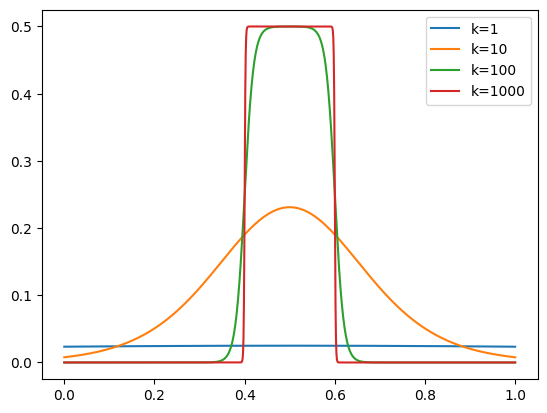
\includegraphics[scale=0.6]{img/bump_functions_1d.png}
      \caption{Bump function approximated with $a = 0.4, b = 0.6$, with differing values of $k$. } 
      \label{fig:bump_functions_1d}
    \end{figure}
  \end{example}

  \begin{example}[Bump Functions in $\mathbb{R}^2$]
    To do this for a 2-D step function, of the form 
    \begin{equation}
      f(x_1, x_2) = \begin{cases} 1 \text{ if } a < x_1 < b \\ 0 & \text{ if else} \end{cases}
    \end{equation}
    this is a simple extension of the first one. We just don't need to make our linear combination dependent on $x_2$ and we're done.
    \begin{equation}
      f(x) \approx \frac{1}{2} \sigma \big( k( x_1 - a)\big) - \frac{1}{2} \sigma \big( k (x_1 - b) \big)
    \end{equation}
  \end{example} 

  \begin{example}[Tower Functions in $\mathbb{R}^2$] 
    Now to construct a tower function of the form 
    \begin{equation}
      f(x_1, x_2) = \begin{cases} 1 & \text{ if } a_1 < x_1 < b_1, a_2 < x_2 < b_2 \\ 0 & \text{ if else} \end{cases}
    \end{equation}
    we need slightly more creativity. Now we can approximate it by doing 
    \begin{equation}
      f(x) \approx \sigma \bigg( k_2 \big[ \sigma\big( k_1 (x_1 - a_1)\big) - \sigma\big( k_1 (x_1 -b_1)\big) + \sigma \big( k_1 (x_2 - a_2)\big) - \sigma\big(k_1 (x_2 - b_2)\big)  big] - b_2\bigg)
    \end{equation}
  \end{example} 

  At this point, we can see how this would extend to $\mathbb{R}^n$, and by isolating parts of the network we can have it approximate tower functions that are completely separate from each other, at any height, and then finally take a linear combination of them to approximate the original function of interest.  

  \begin{theorem}[CS671 Fall 2023 PS5]
    Suppose you have a 2D, $L$-lipschitz function $f(x_1, x_2)$ defined on a unit square ($x_1, x_2 \in \left [0,1 \right ]$). You want to approximate this with an arbitrary neural net $\Tilde{f}$ such that
    \begin{equation}
      \sup_{x \in [0, 1]^2} |f(x) - \Tilde{f}(x)| \leq \epsilon
    \end{equation}
    If we divide the square into a checkerboard of $K \times K$ nonoverlapping squares, approximate the restriction of $f$ to each subsquare with a tower function, what is the least $K$ we would need to ensure that the error is less than $\epsilon$? 
  \end{theorem} 

\subsection{Parameter Symmetry}

  Early in the development of the theory of neural nets, An Mei Chen, (currently VP of engineering in Qualcomm) showed in \cite{symmetry} that for certain neural networks, there are multiple parameters $\theta$ that map to the same function $f$. 

  \begin{theorem}[Parameter Symmetry]
    Consider a 2-layer feedforward network of form 
    \begin{equation}
      f = W^{[2]} \circ \sigma \circ W^{[1]}
    \end{equation} 
    where $\sigma = \tanh$. Let $z$ be the hidden vector. We can see that by changing the signs of the $i$th row of $W^{[1]}$, $z_i$'s sign will be flipped. From the properties that $\tanh$ is an odd function (i.e. $\tanh(-x) = - \tanh(x)$), therefore the activation will be also sign-flipped, but this effect can be negated by flipping the $i$th column of the $W^{[2]}$. Therefore, given that $z \in R^{N}$, i.e there are $N$ hidden units, we can choose any set of row-column pairs of the weight matrices to invert, leading to a total of $2^N$ different weightings that produce the same function $f$. 

    Similarly, imagine that we permute the columns of $W^{[2]}$ and rows of $W^{[1]}$ in the same way. Then this will also lead to an invariance in $f$, and so this leads to $N! 2^N$ different weight vectors that lead to the same function! 
  \end{theorem}

\subsection{Smoothness} 

  Given that the input dimension is $D$, say that all the hidden layers are of dimension $D$ and we have $L$ layers. Then, we are storing a matrix (plus bias vector) at each layer, resulting in a scaling of $O(D^2 L)$. This quadratic scaling leads to overparameterized models, which should raise a red flag. This naturally leads to overfitting, but a strange phenomenon occurs.\footnote{I found this from Lex Fridman's podcast with Ilya Sutskever.}  
  \begin{enumerate}
    \item In the beginning, the training loss goes down along with the validation loss. 
    \item Soon the validation loss starts to go up while the training loss goes down, leading to overfitting. 
    \item The overfitting is worst when the training loss is $0$. 
    \item At this point, the training loss remains at $0$, but generalization starts to improve, and mysteriously the validation loss starts going down. 
  \end{enumerate}

  There are many theories of why the last step ever happens. To interpret this, let's revisit what overfitting means. It means that small perturbations of the inputs will result in large variances in the outputs. If we generalize well, $x + \epsilon$ should also result in $f(x) + O(\epsilon)$. Therefore, this means that the more parameters it has, the better this stability is and therefore the more robust the model. How should we measure this sense of stability? In analysis, a metric to assess the robustness of a deep neural net $f_\theta: \mathbb{R}^n \longrightarrow \mathbb{R}^m$ is its Lipshitz constant, which effectively bounds how much $f$ can change given some change in $x$. 

  \begin{definition}[Lipshitz Continuity]
    A function $f: \mathbb{R}^n \longrightarrow \mathbb{R}^m$ is called \textbf{Lipshitz continuous} if there exists a constant $L$ such that for all $x, y \in \mathbb{R}^n$
    \begin{equation}
      ||f(x) - f(y)||_2 \leq L ||x - y||_2
    \end{equation}
    and the smallest $L$ for which the inequality is true is called the \textbf{Lipshitz constant}, denoted $\mathrm{Lip}(f)$. 
  \end{definition}

  \begin{theorem}[Lipschitz Upper Bound with Operator Norm of Total Derivative]
    If $f: \mathbb{R}^n \longrightarrow \mathbb{R}^m$ is Lipschitz continuous, then 
    \begin{equation}
      \mathrm{Lip}(f) = \sup_{x \in \mathbb{R}^n} ||D_x f||_{\mathrm{op}}
    \end{equation}
    where $||\cdot ||_{\mathrm{op}}$ is the operator norm of a matrix. In particular, if $f$ is scalar-valued, then its Lipschitz constant is the maximum norm of its gradient on its domain 
    \begin{equation}
      \mathrm{Lip}(f) = \sup_{x \in \mathbb{R}^n} ||\nabla f(x)||_2
    \end{equation}
  \end{theorem}

  The above theorem makes sense, since indeed the stability of the function should be equal to the stability of its "maximum" linear approximation $D_x f$. 

  \begin{theorem}[Lipschitz Upper Bound for MLPs]
    It has already been shown that for a $K$-layer MLP
    \begin{equation}
      h_\theta (\mathbf{x}) \coloneqq \mathbf{T}_K \circ \boldsymbol{\rho}_{K-1} \circ \mathbf{T}_{K-1} \circ \cdots \circ \boldsymbol{\rho}_1 \circ \mathbf{T}_1 (\mathbf{x})
    \end{equation}
    the Lipshitz constant for an affine map $\mathbf{T}_k (\mathbf{x}) = M_k \mathbf{x} + b_k$ is simply the operator norm (largest singular value) of $M_k$, while that of an activation function is always bounded by some well-known constant, usually $1$. So, the Lipshitz constant of the entire composition $h$ is simply the product of all operator norms of $M_k$. 
  \end{theorem}

  What about $K$-computable functions in general? That is, given a function $f: \mathbb{R}^n \longrightarrow \mathbb{R}^m$ with 
  \begin{align}
    v_0 (\mathbf{x}) & = \mathbf{x} \\ 
    v_1 (\mathbf{x}) & = g_1 \big(v_0(\mathbf{x}) \big) \\
    v_2 (\mathbf{x}) & = g_2 \big(v_0(\mathbf{x}), v_1 (\mathbf{x}) \big) \\ 
    \ldots & = \ldots \\
    v_k (\mathbf{x}) & = g_k \big(v_0 (\mathbf{x}), v_1(\mathbf{x}), \ldots, v_{k-1} (\mathbf{x}) \big) \\
    \ldots & = \ldots \\
    v_K (\mathbf{x}) & = g_K \big(v_0(\mathbf{x}), v_1 (\mathbf{x}), \ldots, v_{K-2}(\mathbf{x}), v_{K-1}(\mathbf{x}) \big)
  \end{align}
  where $v_k: \mathbb{R}^n \longrightarrow \mathbb{R}^{n_k}$, with $n_0 = n$ and $n_K = m$, and 
  \begin{equation}
    g_k : \prod_{i=0}^{k-1} \mathbb{R}^{n_i} \longrightarrow \mathbb{R}^{n_k}
  \end{equation}
  To differentiate $v_k$ w.r.t. $\mathbf{x}$, we can use the chain rule, resulting in the total derivative 
  \begin{equation}
    \underbrace{\frac{\partial v_k}{\partial \mathbf{x}}}_{n_k \times n} = \sum_{i=1}^{k-1} \underbrace{\frac{\partial g_k}{\partial v_i}}_{n_k \times n_i} \, \underbrace{\frac{\partial v_i}{\partial \mathbf{x}}}_{n_i \times n}
  \end{equation}

  Therefore, it is this Lipschitz property that might entail how stable an MLP is. We have seen from the universal approximation theorems that for a data set of any size, we can always fit a one-layer perceptron that perfectly fits through all of them, given that the layer is large enough. In these cases, we are interested in fitting the data \textit{smoothly}, and theoretical research in bounding the Lipschitz constant is popular.

  In practice this behavior is reflected in \textit{most} cases, but they may be very sensitive in some cases, which we call \textit{adversarial examples}. Adversarial examples take advantage of this weakness by adding carefully chosen perturbations that drastically change the output of the network. Adversarial machine learning attempts to study these weaknesses and hopefully use them to create more robust models. It is natural to expect that the precise configuration of the minimal necessary perturbations is a random artifact of the normal variability that arises in different runs of backpropagation learning. Yet, it has been found that adversarial examples are relatively robust, and are shared by neural networks with varied number of layers, activations or trained on different subsets of the training data. This suggest that the deep neural networks that are learned by backpropagation have \textit{intrinsic} blind spots, whose structure is connected to the data distribution in a non-obvious way. 

